\documentclass[a4paper]{article}
\usepackage{graphicx}
\usepackage{indentfirst}
\usepackage{fancyhdr}
\usepackage{url}
\usepackage[colorlinks=true,linkcolor=blue,filecolor=blue,urlcolor=blue]{hyperref}
\usepackage[top=30truemm,bottom=30truemm,left=25truemm,right=25truemm]{geometry}

\pagestyle{fancy}
\fancyhf{}
\rhead{\thepage}
\lhead{PFS Operational Plan}
\rfoot{}

\title{Subaru Prime Focus Spectrograph (PFS) Operational Plan}
\author{Kiyoto Yabe (Kavli IPMU)}
%%\date{}

\begin{document}
\maketitle
\tableofcontents

\clearpage
%%%%%%%%%%%
%% Background %%
%%%%%%%%%%%
\section{Background}
PFS is an open use instrument of the Subaru Telescope starting its commissioning from 2018 and the scientific operation from 2019. In this document, we describe the operational plan of PFS system during the commissioning phase and after the scientific operation starts. One of the aims of writing this document is not only to define the overall concept of the operation but also to check the possibility of the discontinuity between the operational concept and the telescope system in the Subaru Telescope (including Gen2 and archival system such as STARS/MSTARS) through conversations between the observatory and the PFS project team to mitigate the risk after the commissioning starts. Therefore, some descriptions in this document is of course subject to be updated in the future.

%%%%%%%%%%%%
%% Basic Concept %%
%%%%%%%%%%%%
\section{Basic Concept}
\subsection{PFS System Description\label{sec:pfs_system}}
Here, we briefly summarize PFS instrument system, which is described in the technical documents in more detail. 

PFS is a fiber-fed type spectrograph mounted on the prime focus of the Subaru Telescope. The distinctive features are a wide area of FoV of $\sim1.3$ deg$^{2}$, a large multiplicity of $\sim2400$ fibers, and a wide range of wavelength coverage from 380 nm to 1260 nm. 

PFS comprises several instruments: Prime Focus Instrument (PFI), Fiber system, Spectrograph System (SpS), and Metrology Camera System (MCS). These components are driven independently and sparsely connected in software controlled on the Messaging Hub System (MHS). In the following subsections, a brief summary of each component is described.

\subsubsection{Prime Focus Instrument (PFI)\label{sec:pfs_system:pfi}}
TBW
\subsubsection{Fiber system\label{sec:pfs_system:fib}}
TBW
\subsubsection{Spectrograph System (SpS)\label{sec:pfs_system:sps}}
TBW
\subsubsection{Metrology Camera System (MCS)\label{sec:pfs_system:mcs}}
TBW

\subsection{PFS Survey Operational Concept}
PFS plays an important role as a survey instrument of the Subaru Telescope over the coming years, and thus the observational system should be considered to be optimized in the survey observation. As described in section \ref{sec:survey_operation:software}, PFS software system includes four different software packages, i.e., Survey Planning  \& Tracking software (SPT), Exposure Targeting Software (ETS), Data Reduction Pipeline (DRP), and Instrument Control System (ICS). These systems are ``loosely'' linked to each other with the data exchange via database server \& data archive system, as shown in Figure \ref{fig:pfs_survey_concept}.

\begin{figure}[!htb]
\begin{center}
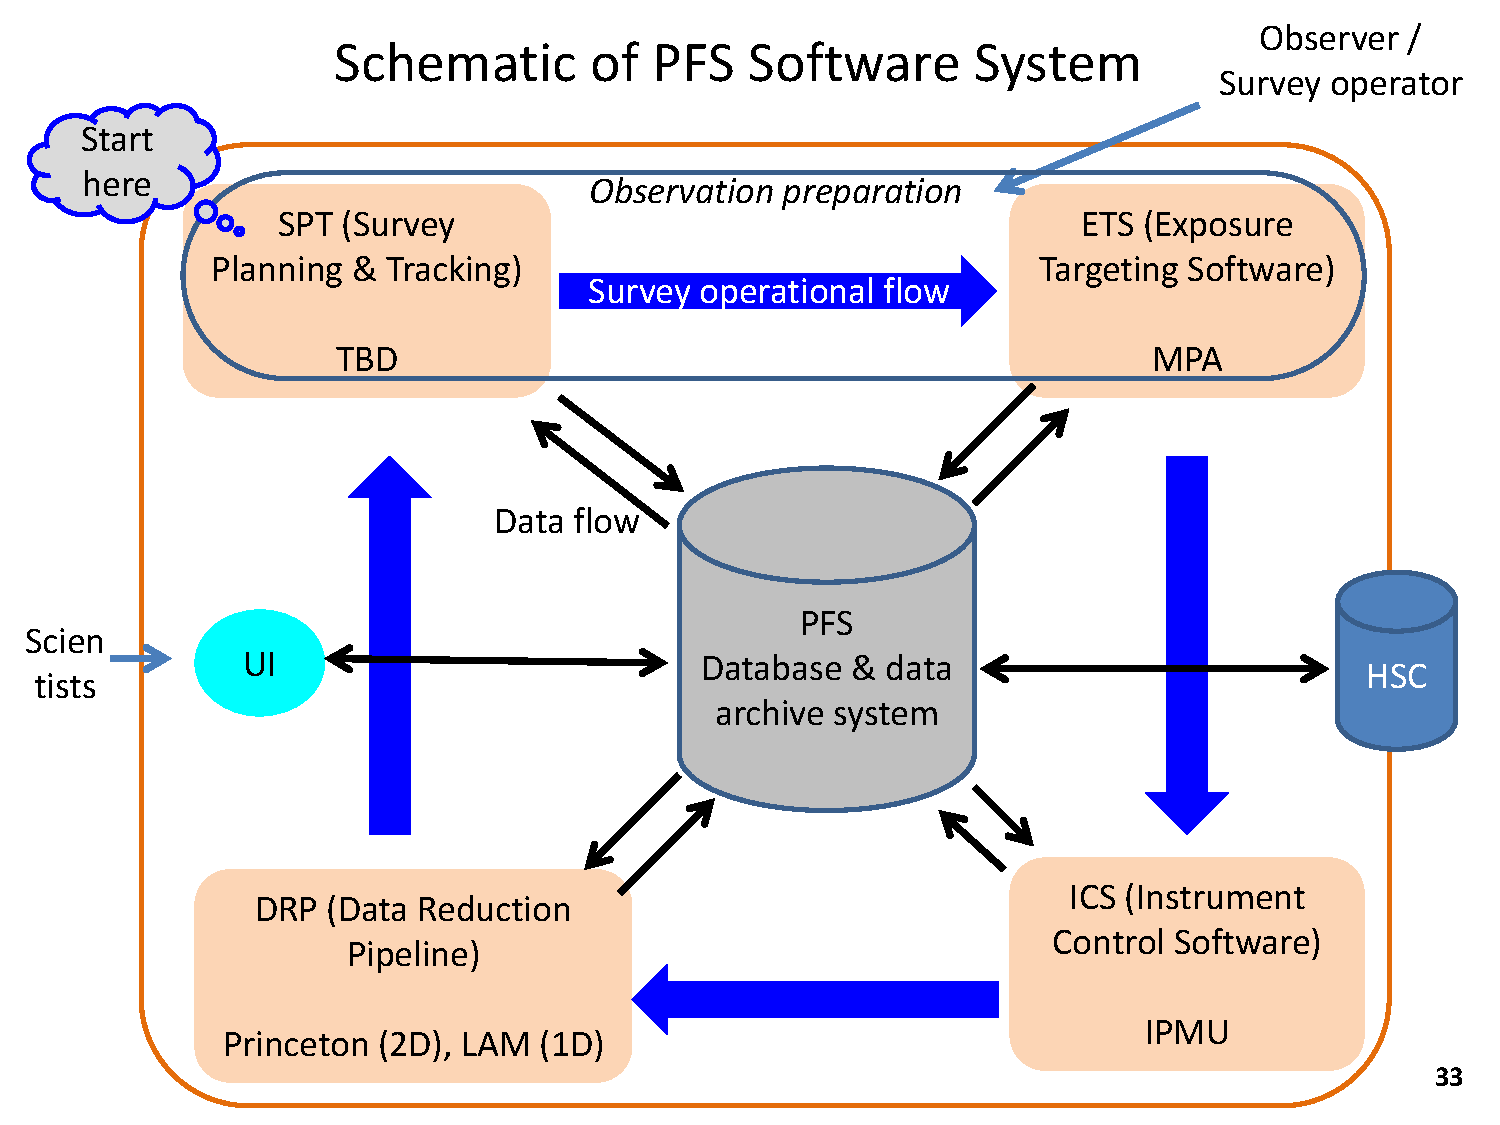
\includegraphics[scale=0.5]{./figures/pfs_survey_operational_concept.pdf}
\end{center}
\caption{The conceptual design of the PFS survey operation including four software packages and database/data archive system. (to be updated)\label{fig:pfs_survey_concept}}
\end{figure}

\subsubsection{Survey Planning \& Tracking software (SPT)\label{sec:survey_operation:spt}}
SPT governs the entire survey planning including the tiling of FoVs with multiple exposures in a series of observing nights. One of the tasks of this system is to track the survey progress and to update the survey planning based on the quality of the obtained spectra providing new targets to ETS. The information on the input catalogue and the obtained data quality used in updating the survey plan are taken from the database and the information on the tiling is also stored in the database server.

\subsubsection{Exposure Targeting Software (ETS)\label{sec:survey_operation:ets}}
ETS is a software to assign fibers to targets provided by SPT and return the optimized fiber configuration in each exposure to be used in the actual observation. 

\subsubsection{Data Reduction Pipeline (DRP)\label{sec:survey_operation:drp}}
DRP conducts the reduction of the obtained 2-dimensional (2D) images into 1-dimensional (1D) spectra with wavelength and flux calibration (2D pipeline). The reduced 1D spectra are passed to a software in which various physical parameters, including redshift, line flux, line velocity, and so on, are extracted from the obtained spectra (1D pipeline). The measured physical quantities are also stored into the database and used in the data quality assurance.

\subsubsection{Instrument Control System (ICS)\label{sec:survey_operation:software}}
ICS is a control system of the PFS hardwares to process fiber configurations (PFI and MCS) and exposures (SpS). The communication between each sub-process is conducted via MHS. The relations between each component are shown in Figure \ref{fig:pfs_software_connections}. 

\begin{figure}[!htb]
\begin{center}
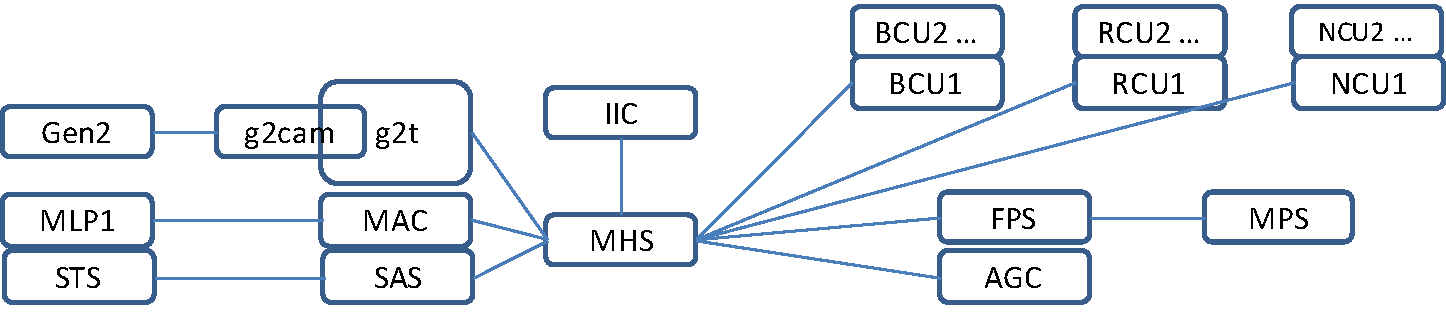
\includegraphics[scale=0.5]{./figures/software_connections.pdf}
\end{center}
\caption{The conceptual scheme of the connections between each system.\label{fig:pfs_software_connections}}
\end{figure}

\subsubsection{Database (inputs from Naoki Yasuda?)\label{sec:survey_operation:database}}
TBW

%%%%%%%%%%%%%
%% Queue operation %%
%%%%%%%%%%%%%
\subsection{PFS operation in queue mode}
TBW (this can be in sec.3?)



%%%%%%%%%%%
%% Detailed Plan %%
%%%%%%%%%%%
\section{Detailed Operational Plan\label{sec:detail_ope_plan}}
%%%%%%%%%%%%%%%
%% Operational sequence %%
%%%%%%%%%%%%%%%
\subsection{The operational sequence during a normal observing run \label{sec:detail_ope_plan:sequence}}

%%%%%%%%%%%%%%%%%%%%%
%% Operational sequence (Definition) %%
%%%%%%%%%%%%%%%%%%%%%
\subsubsection{Definition of operational sequence of PFS observation \label{sec:detail_ope_plan:definition}}
In a normal observing night, the following process can be run:

\begin{itemize}
\item Instrument replacement
\item Startup of the PFS system
\item Telescope pre-check and the PFS status check
\item Telescope focus check
\item Setting up the field with slewing telescope and field acquisition
\item Cobra configuration including reconfiguration in the same field
\item Starting telescope tracking
\item Starting auto guiding system
\item Taking scientific exposures
\item Taking calibration frames
\item Shutdown of the PFS system
\end{itemize}

\noindent Here is the description of each process:\\

\noindent \underline{\textbf{Instrument replacement:}}
\vspace{5pt}

In the beginning of the PFS observing runs, PFS instruments are placed to the right position on the telescope system. Since PFI shares the Popt2 unit with HSC, HSC unit should be replaced from the Popt2 if it is used before the PFS runs. The detailed sequence of this procedure will be described somewhere else.\\

\noindent \underline{\textbf{Startup of the PFS system:}}
\vspace{5pt}

The procedure of the startup mode is done in the following way:

\begin{itemize}
\item Turn the power systems ON
\item Initialize each sub-system
\item Establish the communication between each sub-system via ICS
\item Keep them stable and in stand-by state for the next process
\end{itemize}

The items that DCs should check before pre-check are as follow:
\begin{itemize}
\item ...
\item
\end{itemize}

(TBW in details)\\

\noindent \underline{\textbf{Telescope pre-check and PFS status check:}}
\vspace{5pt}

Once the day-time works of the instrument replacement are completed, the pre-check is needed to be done before the night operation starts. The health check of the PFS instruments are also done during the pre-check procedure. (TBW in details)\\


\noindent \underline{\textbf{Telescope focus check:}}
\vspace{5pt}

The telescope focus check is done after the sun set and the dome opens. The focus check is done by using the image of bright point sources on the PFS AG camera (TBD). This process is also done occasionally during the observations. (TBW in details)\\

\noindent \underline{\textbf{Setting up the field with slewing telescope and field acquisition:}}
\vspace{5pt}

TBW\\

\noindent \underline{\textbf{Cobra fiber configuration:}}
\vspace{5pt}

TBW\\

\noindent \underline{\textbf{Starting telescope tracking:}}
\vspace{5pt}

TBW\\

\noindent \underline{\textbf{Starting auto guiding system:}}
\vspace{5pt}

TBW\\

\noindent \underline{\textbf{Taking scientific frames:}}
\vspace{5pt}

TBW\\

\noindent \underline{\textbf{Taking calibration frames:}}
\vspace{5pt}

TBW\\

\noindent \underline{\textbf{Shutdown of the PFS system:}}
\vspace{5pt}

This process is done under the PFS shutdown mode. The sequence of this process is as below:

\begin{itemize}
\item Stop the current procedure (probably calibration mode?) normally
\item Check the system is in the safe state for shutdown process
\item Turn the power systems OFF (especially PFI and MCS for removal from the telescope)
\end{itemize}

\noindent After the shutdown procedure is done, PFI and MCS is in the stand-by state for the removal from the telescope at the end of each observing run.\\

%%%%%%%%%%%%%%%%%%%%
%% Operational sequence (Overall) %%
%%%%%%%%%%%%%%%%%%%%
\subsubsection{Overall operational sequence of PFS survey observation \label{sec:detail_ope_plan:overall}}

In the actual observing run, the operation is done following the sequence of the processes described in section \ref{sec:detail_ope_plan:definition}. Figure \ref{fig:operation_sequence_overall1} shows the flow chart of the sequence in a typical observing run. Here we assume that the instrument is placed on the Telescope system, that means the starting point is the system startup. In Figure \ref{fig:operation_sequence_overall2}, we show the rough operational sequence in a typical normal observing night. 

Once the startup of the PFS instruments is done, pre-check and PFS health check process is executed during the day-time. After this process is done and the sun sets, then the initial telescope focus check is made after opening the telescope dome. Then, the field set-up procedure slewing the telescope to the target field and the field acquisition procedure by using AG camera are executed. The fiber configuration process runs with the feedback from the acquired image of the back-illuminated fibers on MCS. Although we did not quantified how the movement of the telescope affects the accuracy of the fiber configuration, the fiber configuration process can run in parallel with the telescope slewing and field acquisition procedure if the effect is not significant. Then, the first exposure starts after starting telescope tracking and auto-guiding. 

In most cases of the PFS survey observation, multiple exposures for the same targets and fiber configuration are assumed. In the current operation strategy, we redo the fiber configuration before the next exposure starts. Since the allowable range of the instrument rotator angle is limited ($\pm 60$ deg.), we need to rewind the rotator if the rotator angle hits the limit by 60 or 120 deg. (See \ref{appendix:documents:yabe}). Figure \ref{fig:operation_sequence_overall2} shows an example of the operation over night for a case that observations with multiple exposures in two different fields. In this case, we need to rewind the rotator two times in each field. Since the telescope focus should be varied during a night, we check the telescope focus and apply correction if needed. The frequency of the focus check is not clear at this moment, but we probably need to do a few focus checks during a night. The next sequence of the exposure starts after starting tracking and guiding.

\begin{figure}[!htb]
\begin{center}
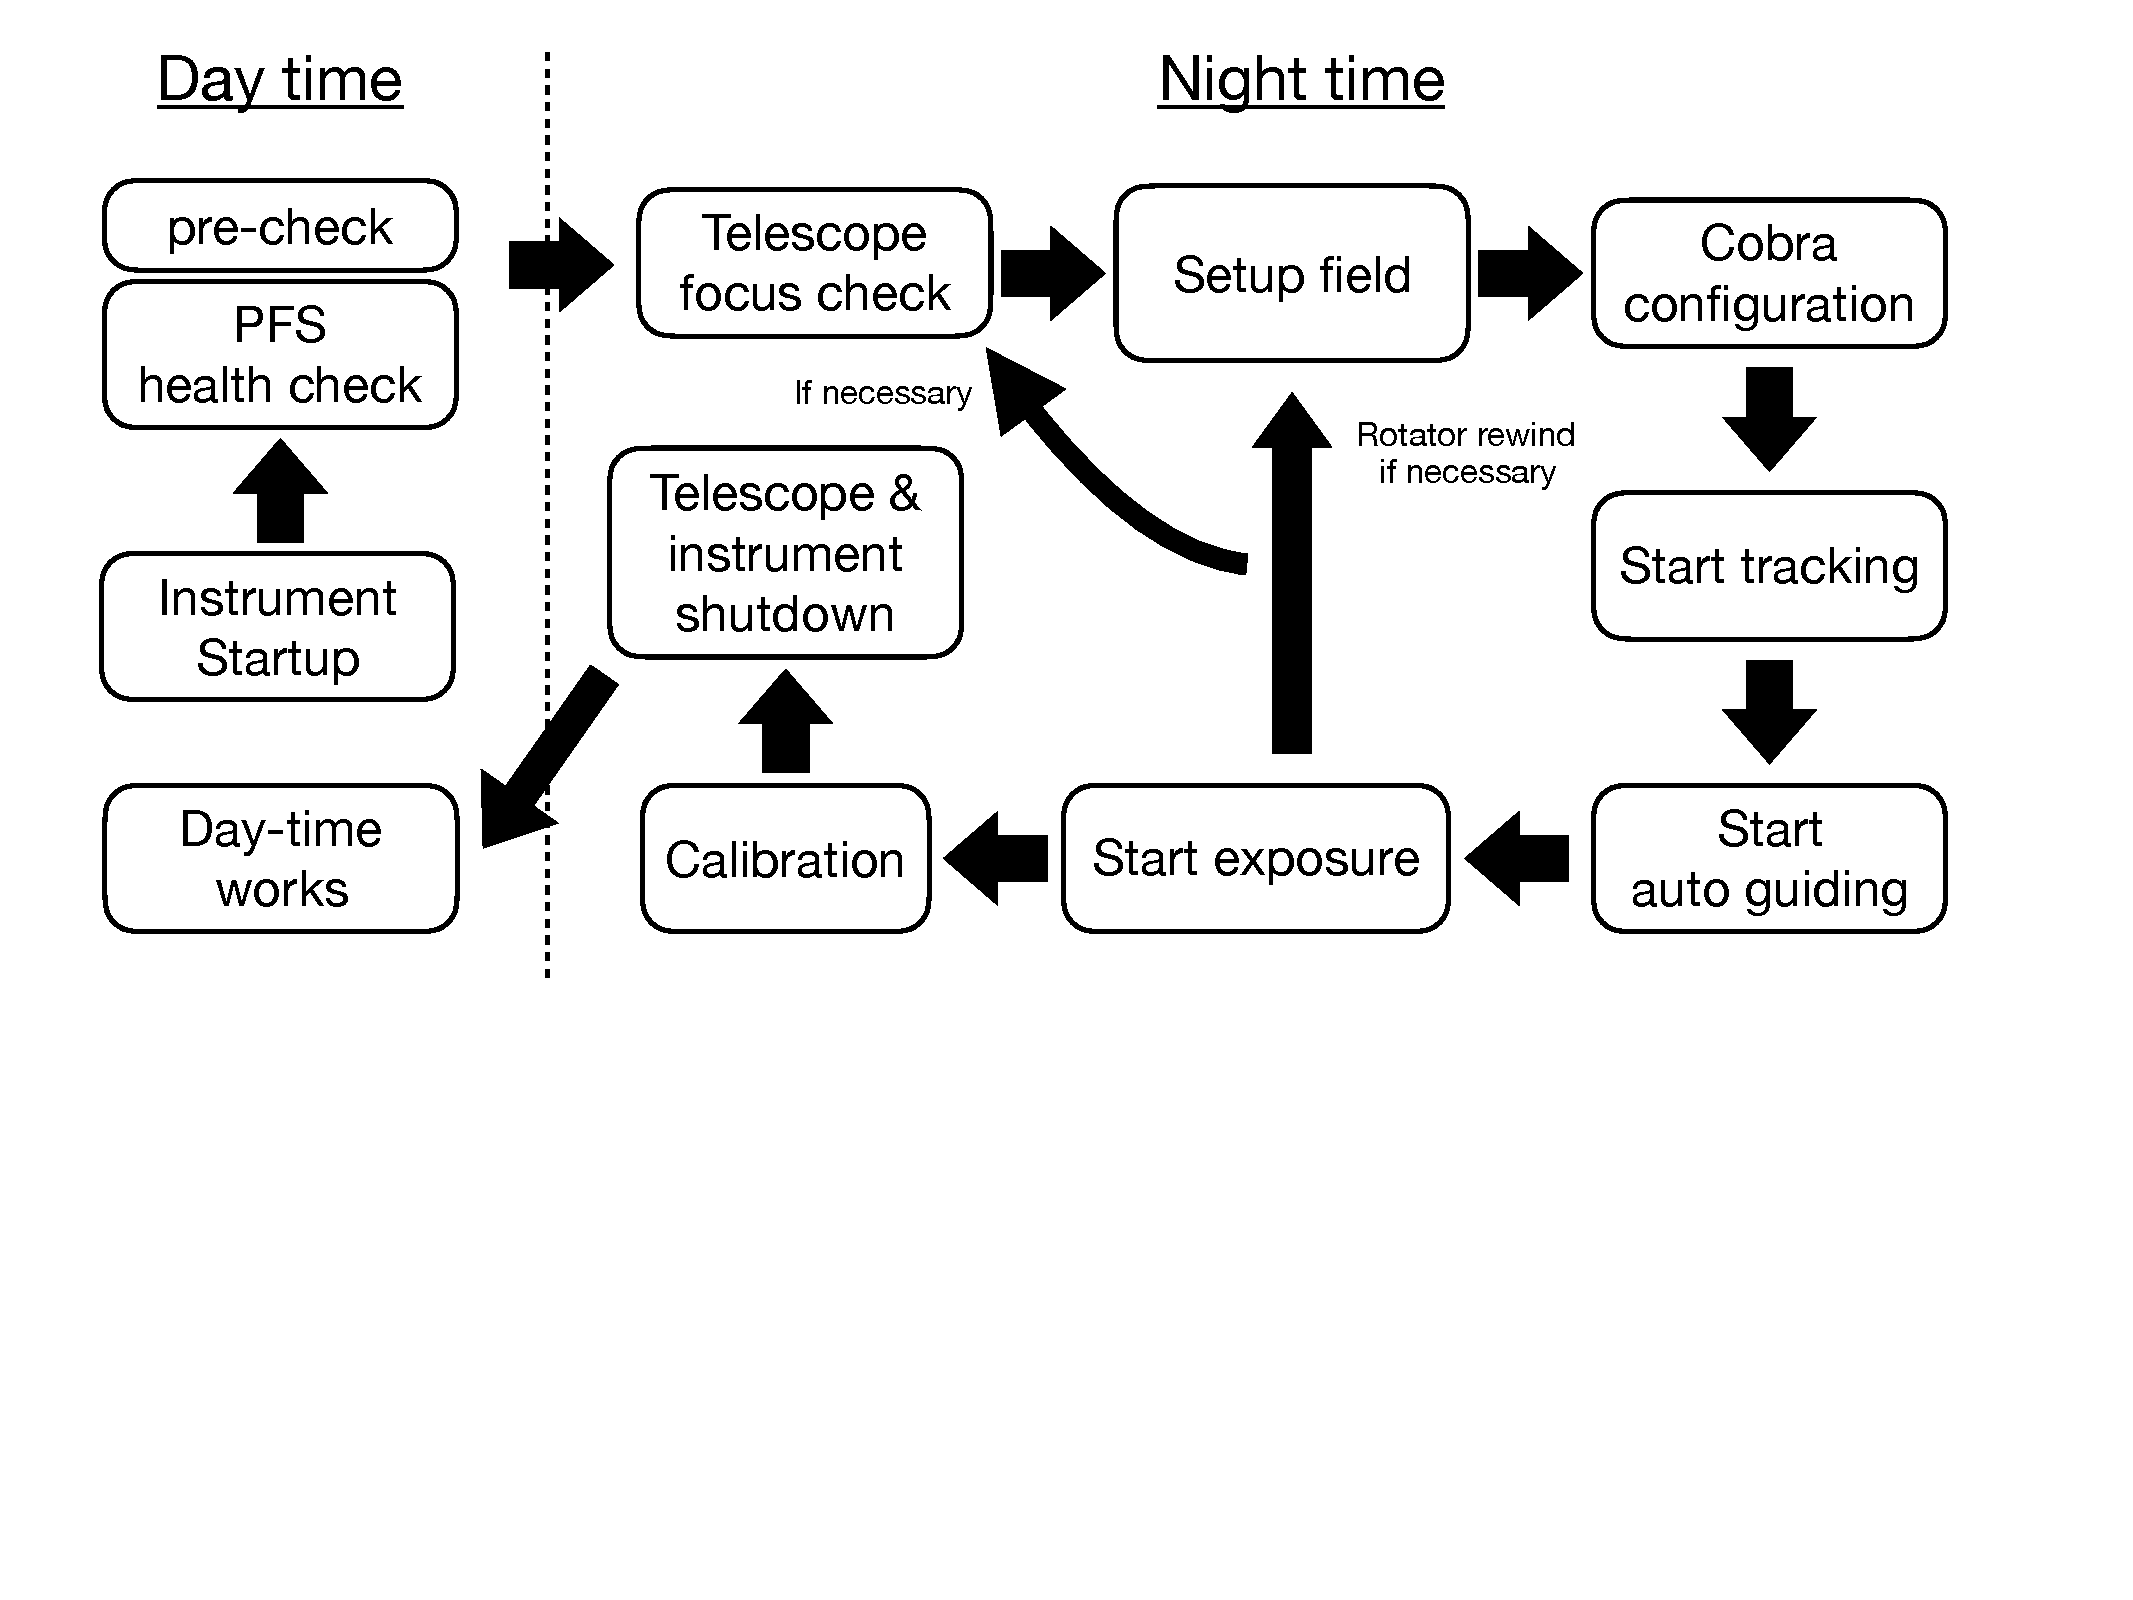
\includegraphics[scale=0.4]{./figures/PFS_night_operation_sequence_overall_cut.pdf}
\end{center}
\caption{An example of the rough operational sequence of the normal scientific observing run. \label{fig:operation_sequence_overall1}}
\end{figure}

\begin{figure}[!htb]
\begin{center}
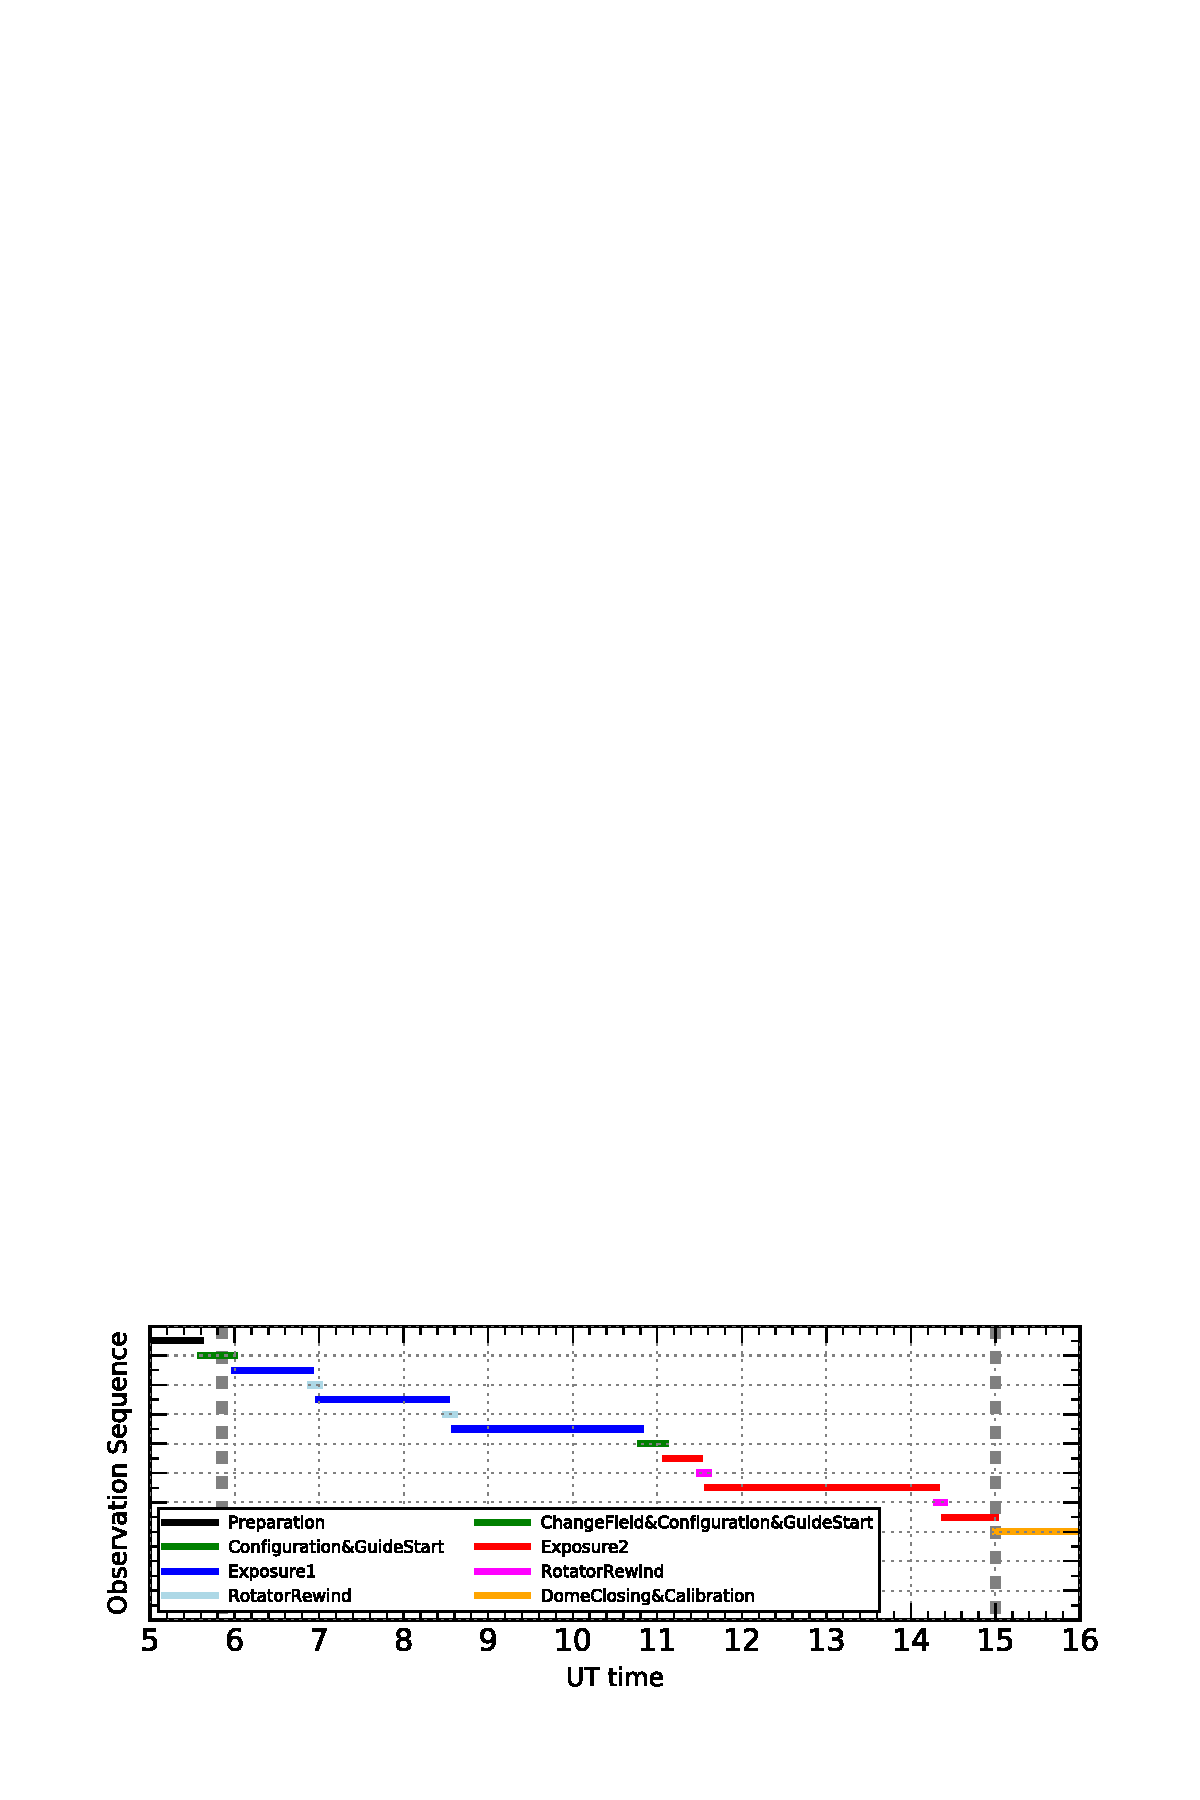
\includegraphics[scale=0.8]{./figures/example_operation_over_night.pdf}
\end{center}
\caption{An example of the time sequence of the normal scientific operation. Here, we assume that moderately long exposures (several hours) are done in two different fields. \label{fig:operation_sequence_overall2}}
\end{figure}

At the end of the night, the calibration procedure is executed after the dome closed. If the PFS observation is continued in the next night, the PFS system may not be required to be in the shutdown mode but in the sleep mode (TBD) in stead.

\begin{figure}[!htb]
\begin{center}
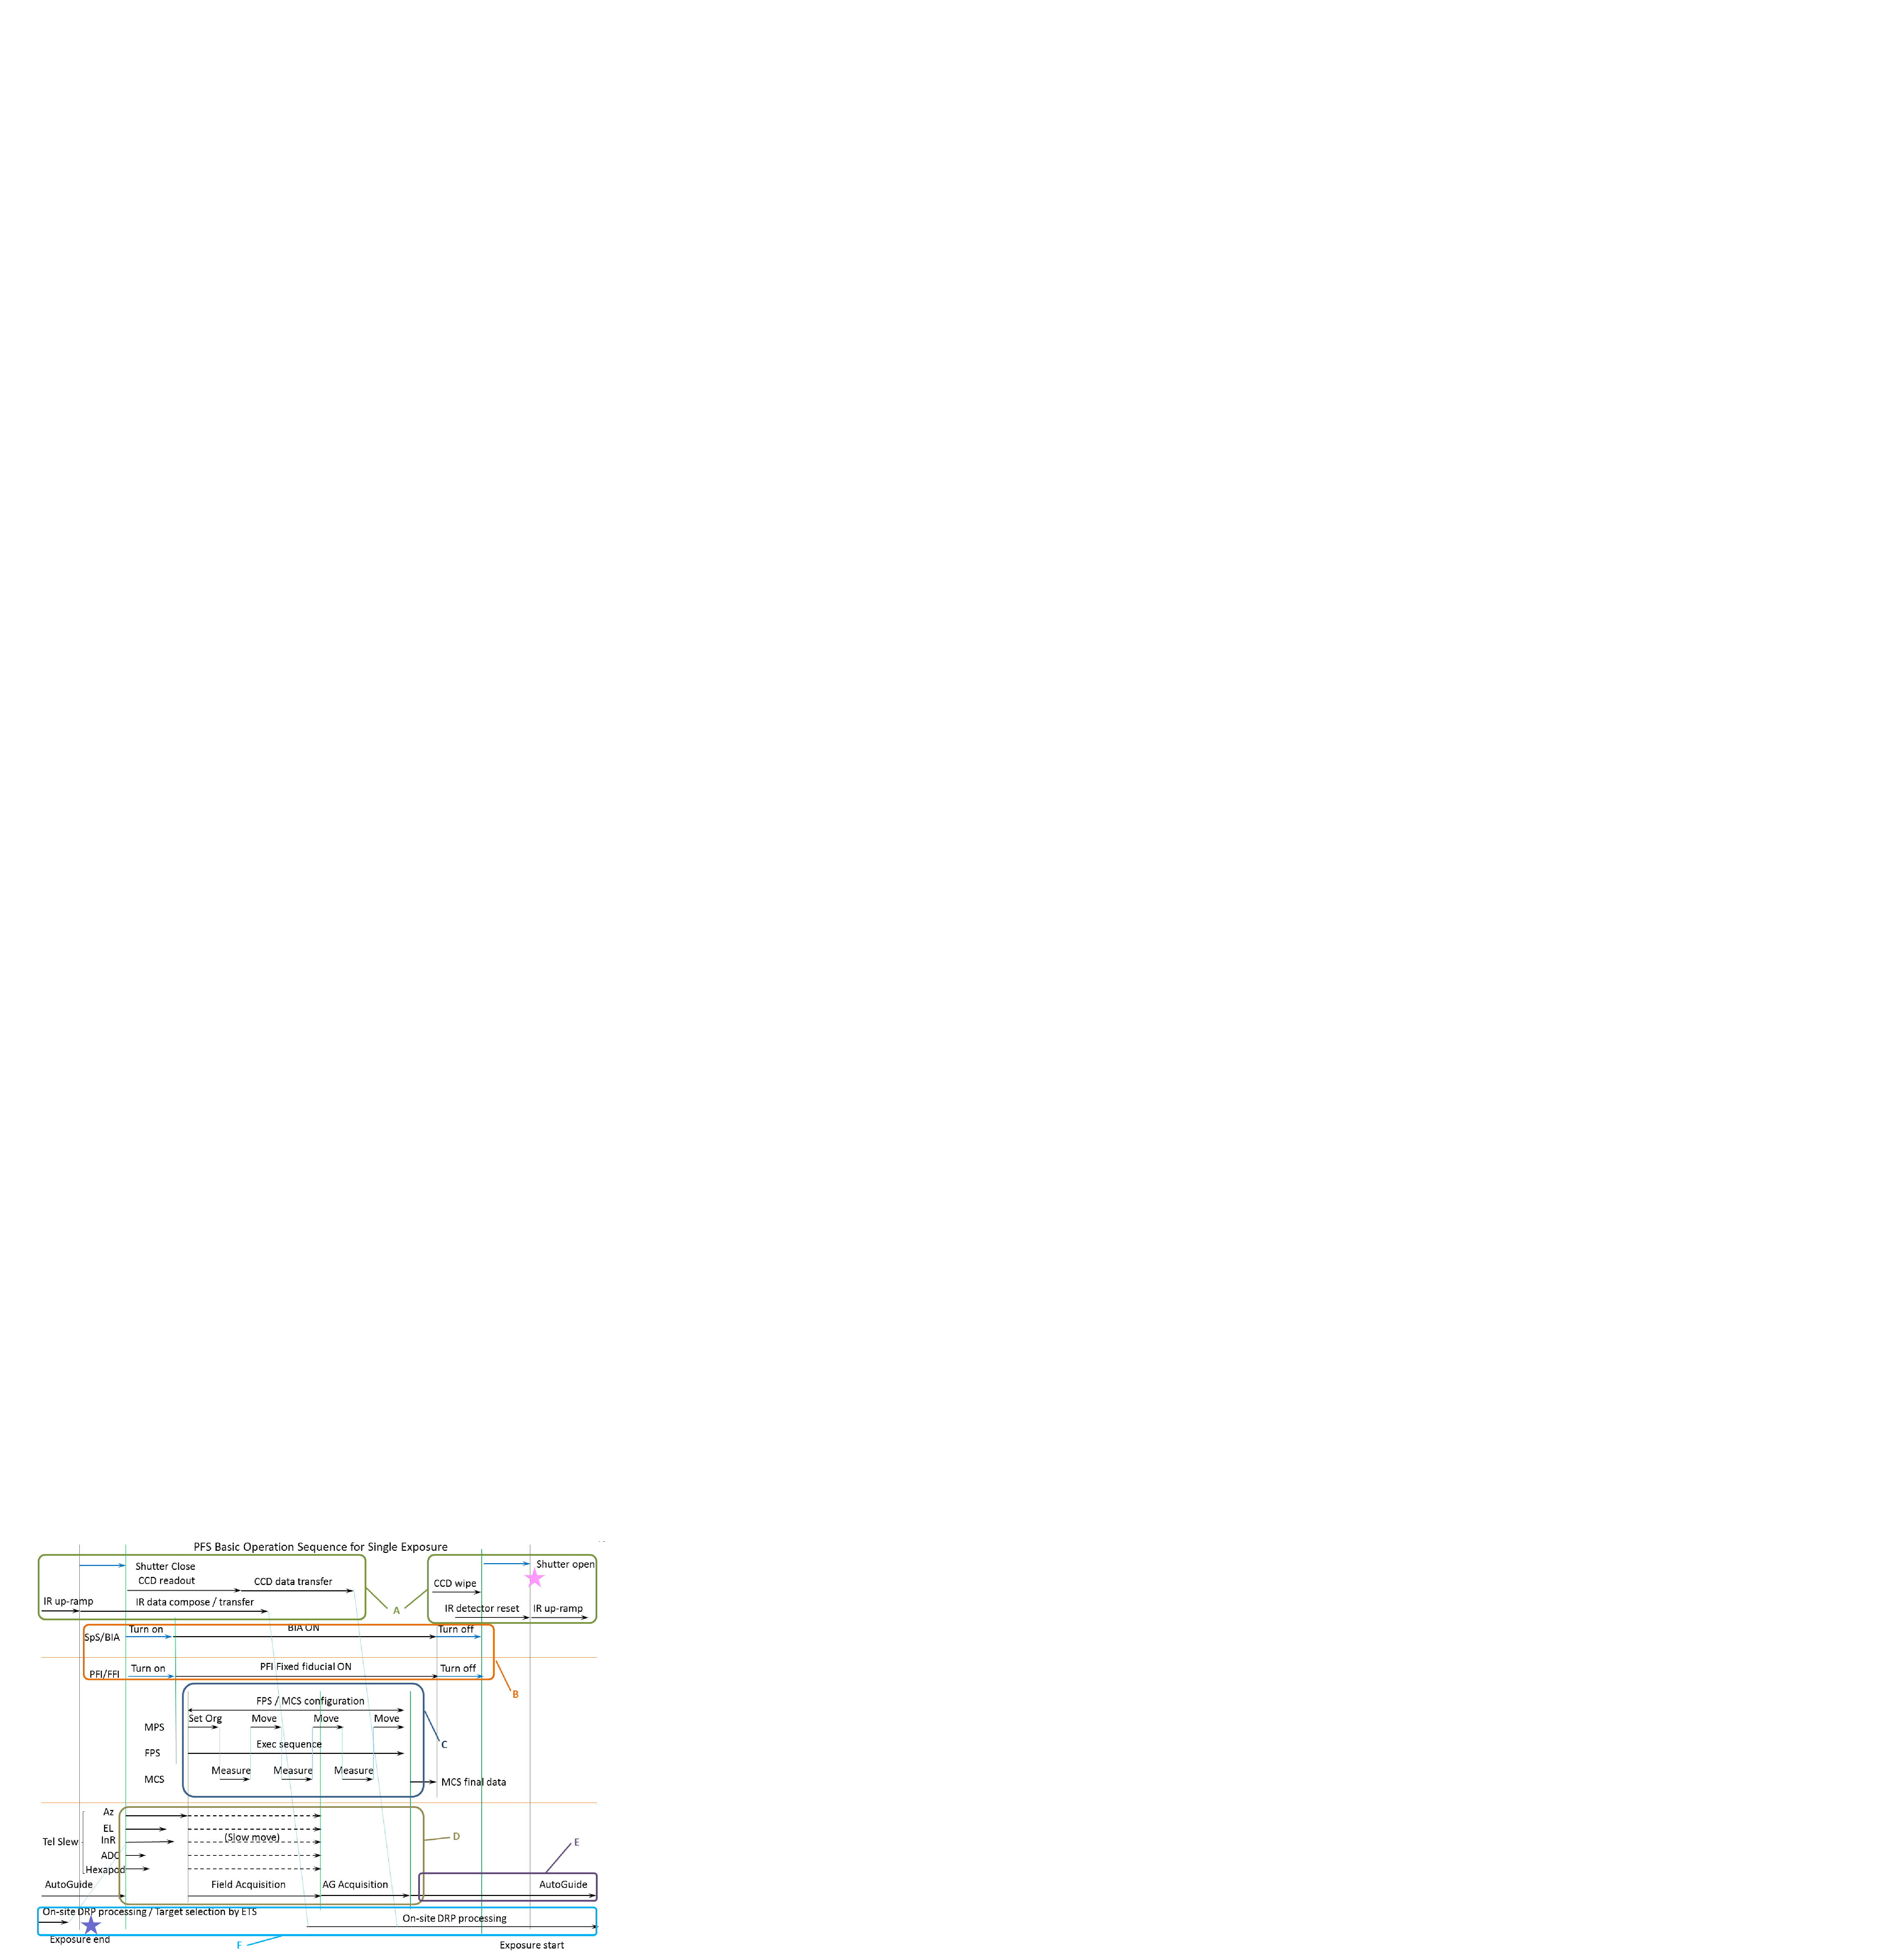
\includegraphics[scale=0.5]{./figures/PFS_Operational_Sequence_for_Single_Exposure_SPIE2016.pdf}
\end{center}
\caption{A schematic view of the operational sequence of instruments as a function of time. (To Be Updated) \label{fig:single_exposure_sequence1}}
\end{figure}

\begin{figure}[!htb]
\begin{center}
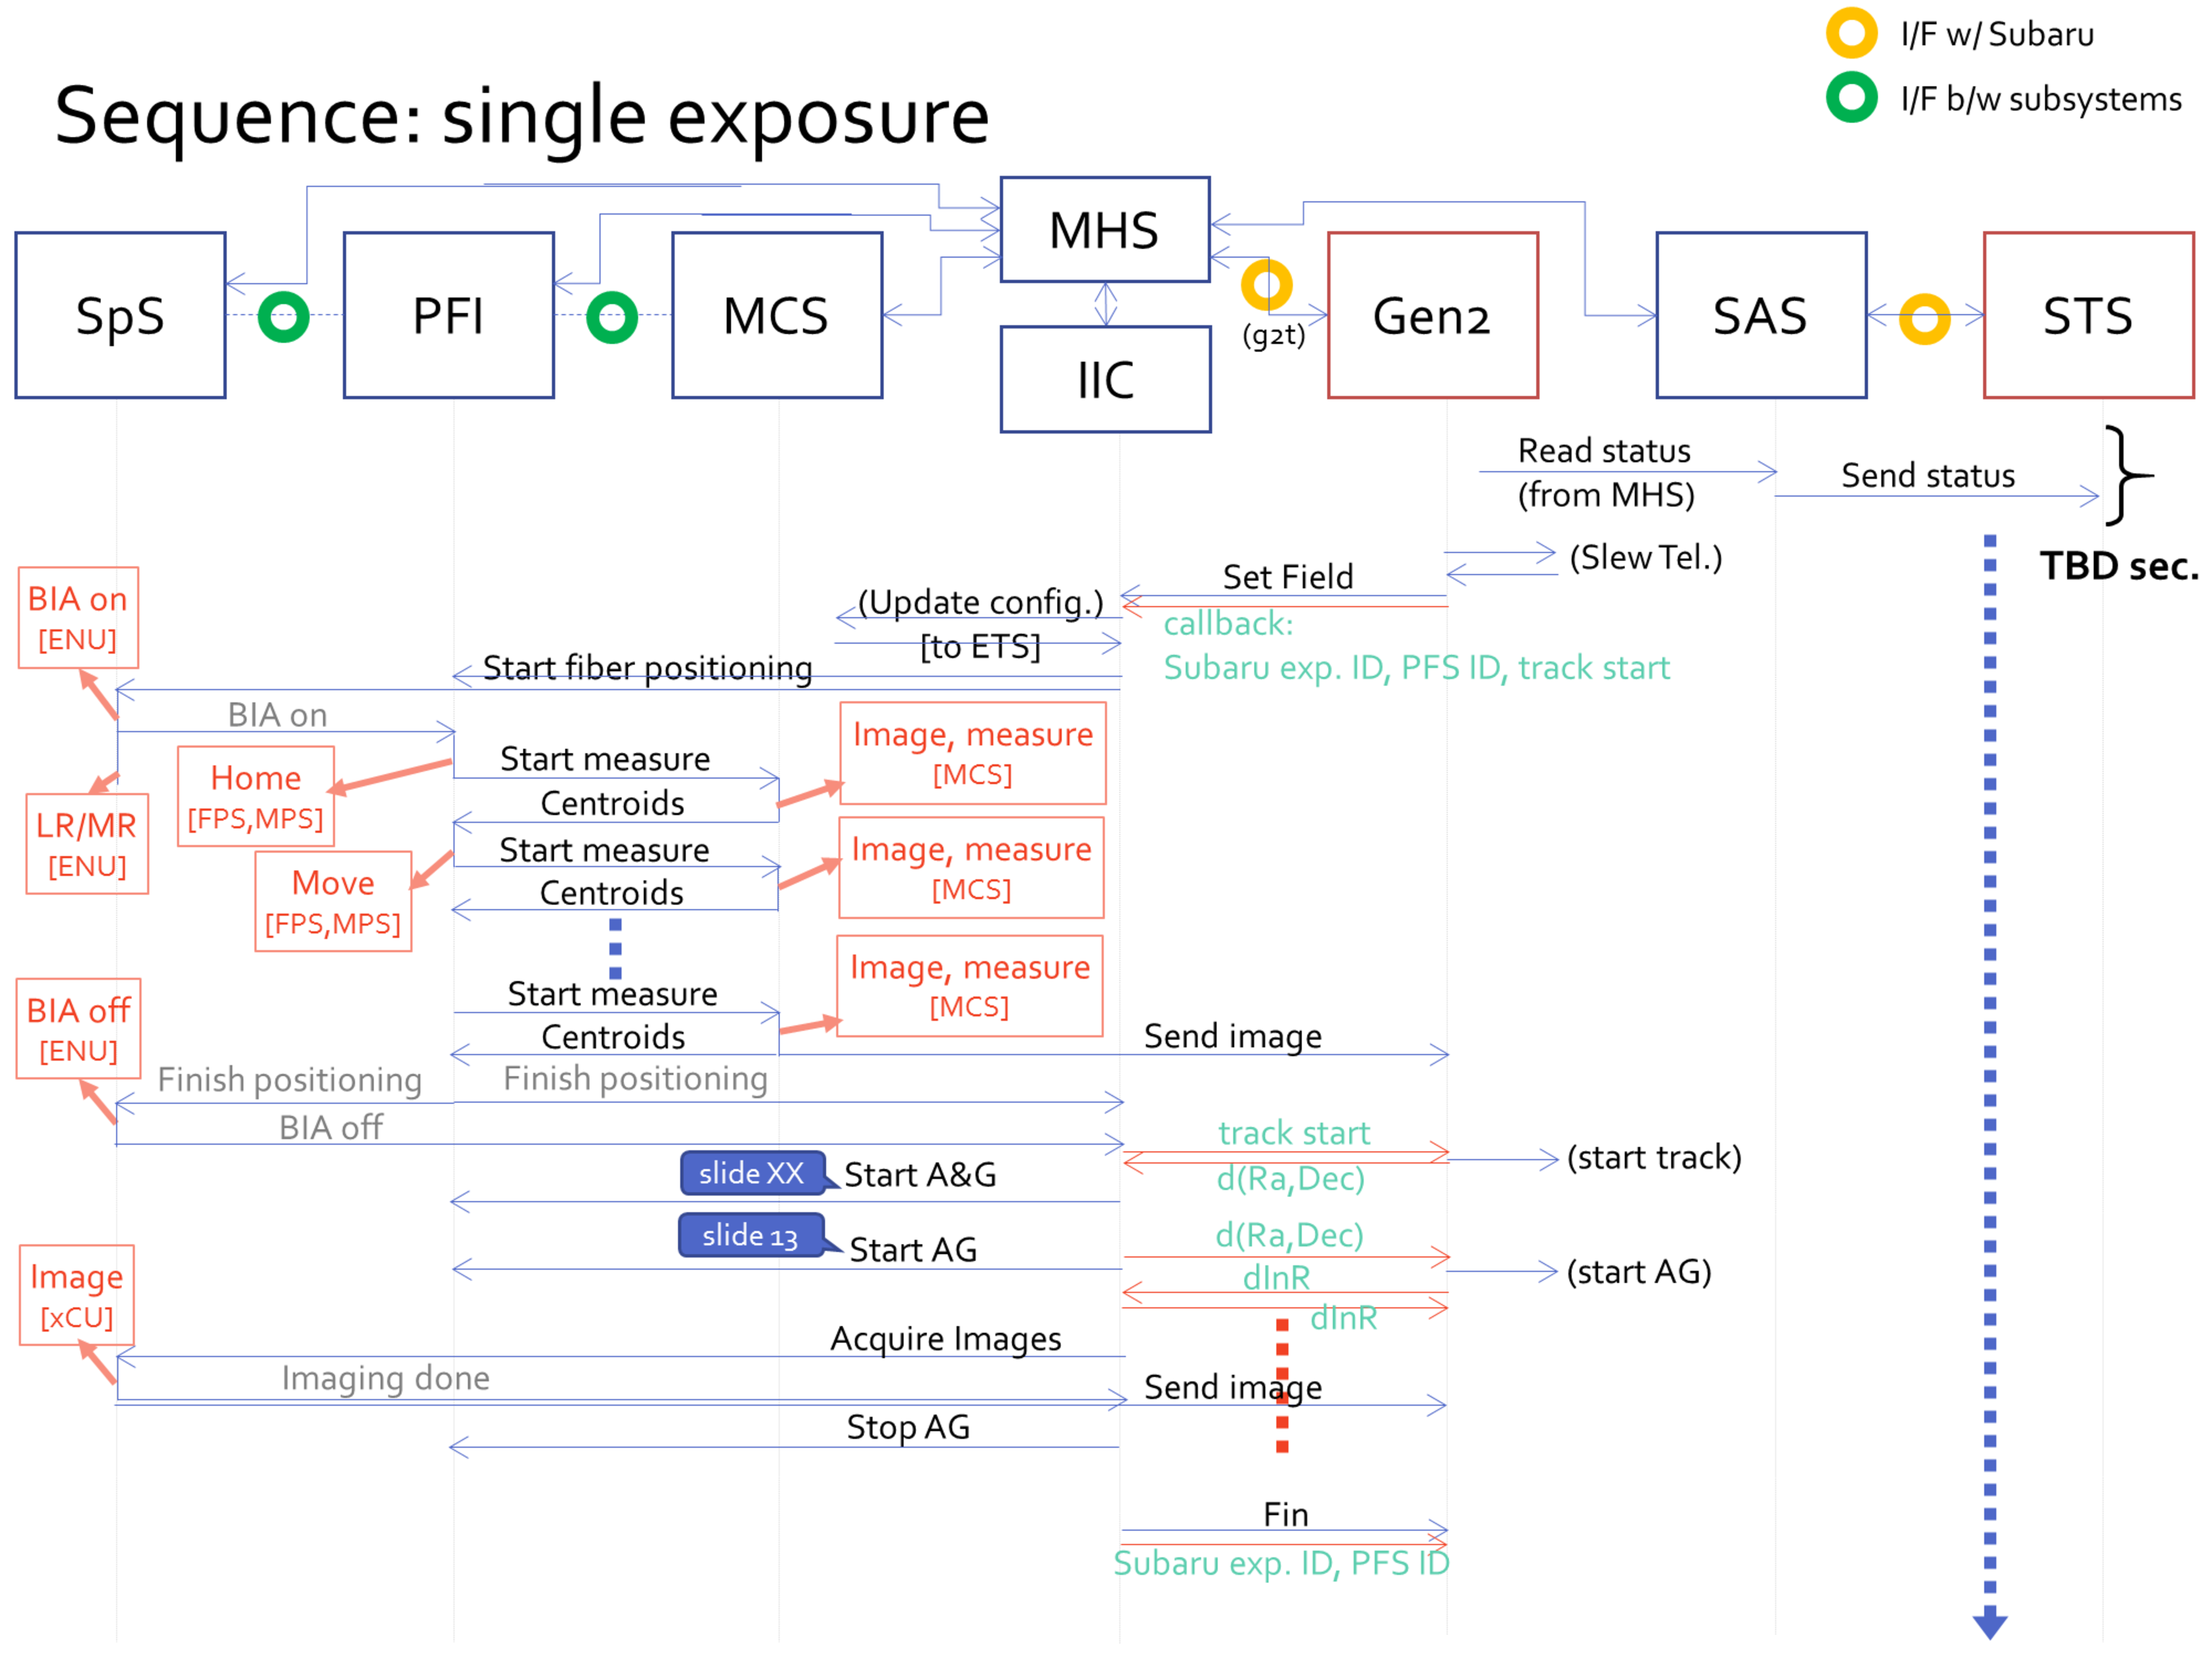
\includegraphics[scale=0.2]{./figures/PFS_sequence_process.pdf}
\end{center}
\caption{A schematic view of the communication between each sub-component during the operation. (To Be Updated)\label{fig:single_exposure_sequence2}}
\end{figure}

As described in \ref{sec:survey_operation:software}, the entire instrument operation is done with sequences associated with each instrumental component. Here we described the detailed processes of each sequence and their relation between each other.

%%%%%%%%%%%%%%%%%%
%% Connection with Tel system %%
%%%%%%%%%%%%%%%%%%
\subsection{Connection between PFS and the telescope systems}
The coordination of the telescope and the instruments at the summit is done by Gen2 system. In the operation of PFS system in the normal observing mode, ICS is required to communicate with Gen2 to receive the telescope status and also send the status of the instrument and requests for the movement to the telescope. The communication between the PFS system (MHS) and the telescope (Gen2) is done via an interface called ``g2t'' by using ``g2cam'' library in Python.

As we mentioned in section \ref{sec:detail_ope_plan:overall}, each sub-sequence can be processed in parallel. Since any commands in g2cam can be triggered only by Gen2, the sequence should be done in the following way:
\begin{itemize}
\item Gen2 prepares a command for callback
\item Once the event occurs, PFS pushes the status with what should be done by Gen2 (such as rotate InR by 120 deg.) and ends the command
\item The sequence running in Gen2 picks up the status value and execute the command
\item Return to the 1st step (if necessary)
\end{itemize}
The detailed processing during the single exposure is described in the section \ref{sec:detail_ope_plan:single}.

Another interface is between the status server called Subaru Telemetry System (STS) and the PFS internal Status Archival System (SAS). Various information on the instrument status is stored in SAS and some of them should also be stored in STS.

%%%%%%
%% QA %%
%%%%%%
\subsection{Checking the quality of the obtained data}
%%%%%%%%%%
%% Summit QA %%
%%%%%%%%%%
\subsubsection{Summit QA of the obtained data (inputs from Robert Lupton?)}
\noindent \underline{\textbf{Initial check of the obtained data:}}
\vspace{5pt}

A monitoring system of the obtained 2D images whether it is a scientific data or not would be helpful for the initial check of the obtained data. This is also useful for the health check of the instrument. The following items should be included in the monitoring system:\\

\begin{itemize}
\item A FITS viewer of the obtained 2D images
\item Measurement of the count level at a given position on the image
\item Zoom-in function for detailed inspections
\item Scale and contrast change for detailed inspections
\end{itemize}

Some functions are already implemented on the current Gen2 system.\\

\noindent \underline{\textbf{Autoguiding monitoring:}}
\vspace{5pt}

The variation of the positional accuracy of assigned fibers to objects is critical to the signal-to-noise ratio of the obtained spectra. The statistical positional errors of the fibers is monitored by the centroids of bright stars in the A/G cameras. Again, bright (point source-like) galaxies can be used for this purpose. Not only the statistics but also a monitoring system with GUI may be useful to observers.\\

\noindent \underline{\textbf{Sky condition monitoring:}}
\vspace{5pt}

The weather condition including seeing and transparency at a given time during the observation is essential to the precise measurements of fluxes of the obtained spectra. Bright stars in the A/G cameras are used for the monitoring of the weather condition. If we have too few stars in the FoVs of the A/G cameras, we alternatively use bright galaxies (as point source-like as possible) for these purposes. FWHM of the object image at a given time is at lease required to quantify the seeing size. The difference between the obtained fluxes and the catalogue values is used for the monitoring the sky transparency. Here, we expect precise photometry in HSC or SDSS and other catalogues.

Another possibility to monitor the sky condition during the night is to measure the flux level of the obtained spectra of e.g. standard stars in each arm. In particular, monitoring the continuum level of blue arm gives us information on the effect of the moon light, and the flux level of the red and/or NIR arm could be useful to the variation of OH sky lines. At least an interface to show the summary of the quality of the obtained spectra is desirable on the summit system (TBD).\\

%%%%%%%%%%
%% Off-site QA %%
%%%%%%%%%%
\subsubsection{Off-site QA of the obtained data (also inputs from Robert Lupton?)}
TBW

%%%%%%%%%%%%%%%%%%%%%%%%%%%
%% Operational sequence during engineering  %%
%%%%%%%%%%%%%%%%%%%%%%%%%%%
\subsection{The operational sequence during a commissioning, engineering, and other unusual (irregular?) observations \label{sec:detail_ope_plan:engineering}}
TBW

%%%%%%%%%%%
%% Possible trouble %
%%%%%%%%%%%
\subsection{Possible troubles during the operation}
In this section, we describe possible troubles envisioned and the solutions during the operation.
\subsubsection{Possible troubles in general}
\subsubsection{Possible troubles during the system startup/shutdown, the pre-check, and the instrument health check}
\subsubsection{Possible troubles during the scientific operation}
\subsubsection{Possible troubles during the calibration operation}

\clearpage
\appendix
%%%%%%%%%%%%%%%%
%% Pointers to documents %%
%%%%%%%%%%%%%%%%
\section{Pointers to technical documents}

\subsection{Documents by Atsushi Shimono \label{appendix:documents:shimono}}
\begin{itemize}
\item \href{http://sumire.pbworks.com/w/file/102897967/SSN-00011-001-ICSSeq-1-Overall.pptx}{SSN-00011-001} (Study on PFS Observation Sequence (I) Overall)
\item \href{http://sumire.pbworks.com/w/file/94687160/SSN-00012-001-ICSSeq-2-CommandToAG.pptx}{SSN-00012-001} (Study on PFS Observation Sequence (II) From command next field to AutoGuide)
\item \href{http://sumire.pbworks.com/w/file/93138234/SSN-00006-001-AGtoGen2.pptx}{SSN-00006-002} (Study on PFS A\&G/AG communication)
\item \href{http://sumire.pbworks.com/w/file/101124121/SSN-00016-001-Gen2-OBCP.pptx}{SSN-00016-001} (Connection from PFS ICS to Gen2)
\item 
\end{itemize}

\subsection{Documents related to the commissioning by Yuki Moritani\label{appendix:documents:moritani}}
\begin{itemize}
\item \href{}{PFS commissioning plan}
\end{itemize}

\subsection{Documents related to various studies on PFS operation by Kiyoto Yabe\label{appendix:documents:yabe}}
\begin{itemize}
\item \href{http://member.ipmu.jp/kiyoto.yabe/PFS/tmp/material_pfs_operation_dots_20160629.pdf}{material\_pfs\_operation\_dots\_20160629.pdf} (Effects of instrument rotator angle on dot coverage on the focal plane)
\end{itemize}

%%%%%%%%%%%%%%
%% Operation of FMOS %%
%%%%%%%%%%%%%%
\section{The operational process in FMOS}
\subsection{}


\end{document}
